\pagebreak
\section{Problemática}

Una de las cosas que señala \textcite{Jin2023} es que en los circuitos de un
computador se pueden encontrar fallas que se caracterizan principalmente por la
degradación de uso y el estropeo repentino de algún componente. En principio
se piensa que ya se debería tener control de ese aspecto, pero se sigue tratando
de manejar tal situación por la cantidad de demanda por la reparación de
computadores tanto domésticos como empresariales. Además, una de las cosas que
\textcite{Aboaoja2022} aborda sobre la ciberseguridad, que es una de las áreas
más importantes para la protección de la información de los usuarios y que
procura evitar que los sistemas de cómputo tengan fallos

Ambas áreas son enfocadas principalmente debido a su relación que tienen con el
funcionamiento de un equipo de cómputo, ya que si el mismo tiene una deficiencia
en su funcionamiento, bien pueda ser que en la parte física haya un
comportamiento que no deba ocurrir, o que en el software (la parte lógica) tenga 
integrado un elemento que estorbe las acciones que el usuario quiera realizar.
Las situaciones a continuación describen lo que se refiere cuando se habla de
``Inadecuado funcionamiento de un equipo de cómputo'' tanto para dispositivos de
sobremesa como móviles:

\subsection{Situaciones relacionadas con el mal funcionamiento de hardware}

\textcite{Herat2020} informó que en 2019 se observó que alrededor del mundo se
desperdiciaron 53.6 millones de toneladas métricas y que se estimó que para el
2023 se tendrán 74.7 millones de toneladas métricas de desperdicios
electrónicos. Y que anualmente se desechan entre 1 y 10 millones de toneladas
métricas en los países industrializados y los que están en vías de desarrollo
desechan alrededor de 500 mil y un millón de toneladas métricas. Esta
acumulación de dispositivos se generan normalmente por una serie de actitudes
que \textcite{Hartl2023} relacionan con la psicología del mercado cuando las
empresas que fabrican diversos productos que con el paso del tiempo resultan
tener más capacidad, más velocidad y más eficiencia: ``Los bienes duraderos
que se estropean al cabo de un tiempo inducen a los consumidores a comprar uno
nuevo, lo que estimula la demanda de este producto.''

Ante esta situación, Kaliyavaradhan et al. (2022) como se cita en
\textcite{Seif2024} encontraron que esta actitud ocurre principalmente por los
acelerados cambios y avances que presenta la tecnología ante varias de nuestras
actividades cotidianas y laborales, cosa que lleva a directamente hacer
reemplazos constantes debido a las incompatibilidades que presentan las
herramientas de software con los componentes y capacidades del hardware: ``A
medida que entran en el mercado nuevos dispositivos con las últimas
prestaciones, los consumidores se deshacen de los más antiguos, lo que aumenta
las tasas de residuos''

Un aparato electrónico que se estropea de forma inesperada, normalmente uno
podría pensar que el problema viene a través del uso, sin embargo, también se
encontró de acuerdo con \textcite{Hartl2023} que también ocurre por
conveniencia empresarial, ya que si alguien nota que su máquina no funciona
como se espera o deja de ser útil, entonces se cambia para mantener a flote la
economía de la empresa que diseña el producto:

\begin{displayquote}
  Aunque ingenuamente se podría pensar que la vida útil de un producto depende
  normalmente del desgaste de sus materiales más alguna influencia aleatoria,
  también puede ser el resultado de una elección empresarial. La obsolescencia
  planificada significa que las empresas diseñan sus productos de forma que no
  duren mucho.
\end{displayquote}

% Otras cuestiones a tratar
Ahora, en cuanto a los aspectos técnicos sobre las fallas en aspectos de
hardware, en la fabricación se tiene un análisis sobre el funcionamiento del
circuito usando un modelo lógico de fallos y otro de simulación de sistemas. Pero
como somos seres que cometen errores, a la hora de hacer tales análisis se
omiten ciertos datos particulares como la implicación que podrían generar
ciertos componentes tras haber realizado en un componente en particular o el
resultado que se generó tras el diseño de las partes que conforman los equipos
de cómputo. \parencite{Jin2023}

En esto da sentido a lo que expresan \textcite{Zailani2021} cuando se
encuentran con la problemática de que los usuarios que no son experimentados en
la mantención de hardware y deciden tomar las medidas que solo conocen, pero
que resultan ineficientes ante las situaciones que se presentan cuando un
dispositivo tiende a fallar por algún motivo: 

\begin{displayquote}
  A veces, algunos productos informáticos del mercado ofrecen lugares de
  servicio oficiales de difícil acceso, por lo que los usuarios se muestran
  reticentes a repararlos y, al final, prefieren los lugares de servicio
  públicos. Sin embargo, algunos usuarios saben que si reparan su ordenador en
  un lugar público, es arriesgado porque no hay información clara sobre los
  costes de reparación ni sobre los daños.
\end{displayquote}

\subsection{Situaciones relacionadas con las fallas de ciberseguridad}

Por norma general, algunas veces vemos que ``ciberseguridad'' y ``seguridad
informática'' son sinónimos. Sin embargo, la seguridad informática es el área de
proteger la información de los riesgos que conlleva el entorno en donde se
encuentra y que puede tener otros formatos que no siempre están relacionados
con los equipos de cómputo. En cuanto a la ``ciberseguridad'' tiene una cuestión
similar, solo que se especializa en la protección datos almacenados en sistemas
de cómputo; lo que significa que la ciberseguridad hace parte de la seguridad
informática: ``Se entiende que la ciberseguridad tiene como objetivo
principal la protección de la información digital, que está o es transmitida
entre los todos los dispositivos que se encuentran interconectados, por esto,
la ciberseguridad está en la seguridad informática''
\parencite{Mosquera2019} 

Así que reconociendo lo que representa la ``ciberseguridad'' y teniendo en
cuenta que esto se aplica a diversas áreas como lo comenta
\textcite{CanoMartinez2022} de que la seguridad de la información digital es
primordial, ya que si es escasa, se pueden generar desde efectos molestos hasta
destructivos en el aspecto político, económico, legal, etcétera:

\begin{displayquote}
  En este escenario, la ciberseguridad nacional enfrenta diferentes tensiones y
  fuerzas a nivel político, económico, social, tecnológico, legal y ecológico,
  que demandan salir de la postura tradicional de “esperar y ver”, para
  movilizar reflexiones y esfuerzos que permitan “delinear y actuar”.
\end{displayquote}

Sabiendo que en diversos entornos, se pueden encontrar brechas que pueden ser
aprovechables tanto por cualquier persona como de cualquier otro software. Una
de las partes más preocupantes es el hecho de que los ransomware (malware que
cifra datos) sea el tipo de malware que actualmente es uno de los que son más
frecuentes: ``El Netskope Cloud Report de septiembre de 2016 reveló que el
55,9\% de los archivos infectados con malware que se encuentran en las
aplicaciones en la nube se comparten públicamente, por lo que la nube es una
plataforma atractiva para los atacantes.'' \parencite{Rosli2019}

Los mismos demuestran que los problemas en cuanto a malware cada
vez se hacen más notorios, por ejemplo en la Figura~\ref{fig:report2017} se
muestra de forma general la cantidad de incidentes relacionados con la
ciberseguridad en 2018. Y los mismos también comentan que la tasa del malware
aumentó a un 43.5\% del total de los incidentes ocurridos en 2018. Lo que indica
qué tan importante es el de hacer que los usuarios se encuentren con malware.

\begin{figure}[htb]
  \centering
  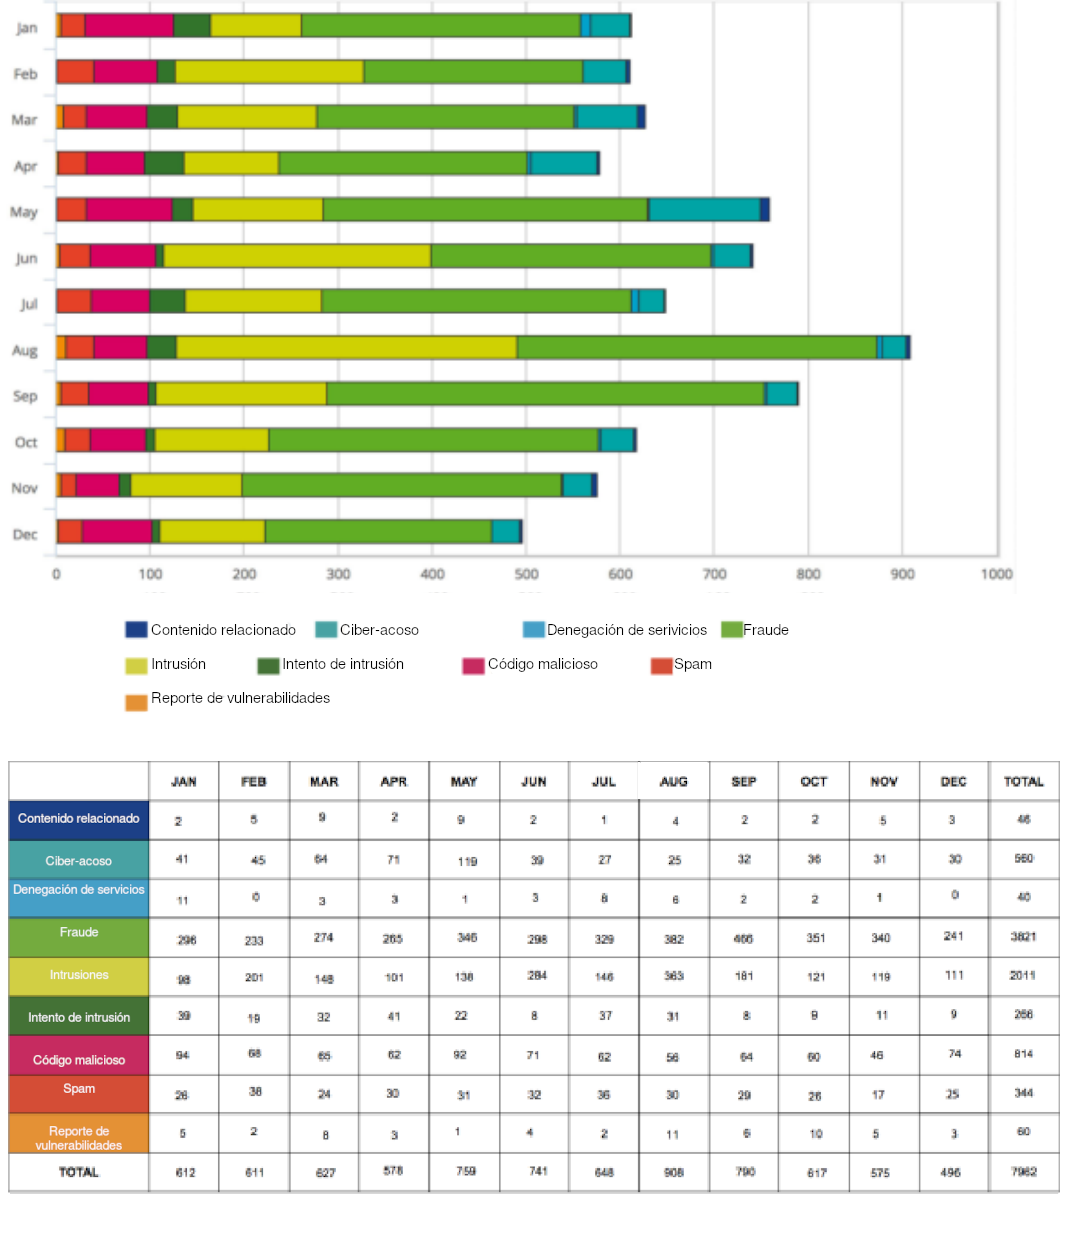
\includegraphics[width=0.75\textwidth]{./pictures/report2017.png}
  \caption{
    \textbf{Nota:} Estadísticas de incidentes reportados en 2017 Tomado de
    \cite{Rosli2019}
  }
  \label{fig:report2017}
\end{figure} 

% Otro problema para otros entornos

\subsubsection{Problemas en el aspecto de los sistemas de salud}

Una de las áreas en las que también se logra presenciar lo comprometidas que se
encuentra la ciberseguridad en los sistemas sanitarios al quedar completamente
expuestos; una prueba realizada por Google, se descubrió que una de sus
inteligencias encontraron y expusieron información crítica tanto de médicos
como de pacientes. Lo que significa que los ``cibercriminales'' pueden realizar
sus objetivos relacionados con el sistema sanitario:

\begin{displayquote}
  Informes aparecidos en el Washington Post y en otros medios de comunicación
  han descrito cómo las asociaciones de Google con el fin de entrenar algoritmos
  de inteligencia artificial dieron lugar inadvertidamente a que algunos datos
  con información sanitaria protegida se cargaran de forma que quedaran
  expuestos a cualquier persona con una capacidad básica de motor de búsqueda.
  \parencite[Wakabayashi D, 2019, como se cita en][]{Banja2020}
\end{displayquote}

También \textcite{Banja2020} destacó que en diversas organizaciones se almacene
información de manera consentida, por lo que si hay fallas de seguridad por
parte de un ente, (no tiene que ser necesariamente un atacante) se compromete
entonces el estado de seguridad de la gente a la que pertenece tal entidad. Y
también 

% Poner sus mejoras
\subsubsection{Problemas en el IoT}

A grandes rasgos, es un campo en el que objetos de uso cotidiano están
conectados a una red, que a su vez, está conectada a internet. A pesar de ser un
campo en el que es poco común en el uso diario, se vuelve completamente
importante en la seguridad informática, ya que como comenta
\textcite{Aboaoja2022}, el desarrollo del malware se volvió tan sofisticado que
los que terminan siendo desarrollados pueden distinguir el tipo de máquina en
la que están, así que no es de extrañar que existan programas que se dispersen
en una red sin el consentimiento de los usuarios.

En el Internet de las Cosas al estar repleto de tantos computadores, se requiere
entonces de una cantidad de recursos masiva para la protección de la información
que se utiliza, y como el malware cada vez se hace más silencioso ante la
protección, cosa que es my peligroso para entidades que usan el IoT de forma
común y se tenga que gastar más 6.000 millones de dólares para sistemas de
protección de la información bastante avanzados:

\begin{displayquote}
  Los informes de Gartner1 y Juniper Research2 sugieren que el gasto mundial en
  seguridad de IoT fue de 1.1 mil millones de dólares y se disparó más de 3.1
  mil millones de dólares en 2021. Además, se prevé que se dispare hasta los
  6.000 millones de dólares en 2023, lo que es un resultado directo del aumento
  de las vulnerabilidades en los sistemas. La discusión anterior nos lleva a
  creer que el diagnóstico y la resolución de fallas en un sistema IoT será un
  gran problema en el futuro cercano, a menos que todas las entidades dentro del
  sistema pertenezcan a la misma empresa. \parencite{Singh2022}
\end{displayquote}

\subsubsection{Situaciones nacionales}

\textcite{CanoMartinez2022} y \textcite{Mosquera2019} muestran lo que ocurre a
nivel nacional sobre el estado de la seguridad informática y no únicamente
viendo los delitos que más se cometieron con respecto a lo que se muestra en la
Figura~\ref{fig:delitos} de acuerdo con la Ley 1273 de 2009 del código penal
nacional. Aunque aquello pone en evidencia que se procura obtener un beneficio
comercial o económico, ellos también evidencian que se realizan para tener una
influencia sobre las actividades comunes. Siendo estas extendidas al uso de las
tecnologías de forma amplia.

\begin{figure}[htb]
  \centering
  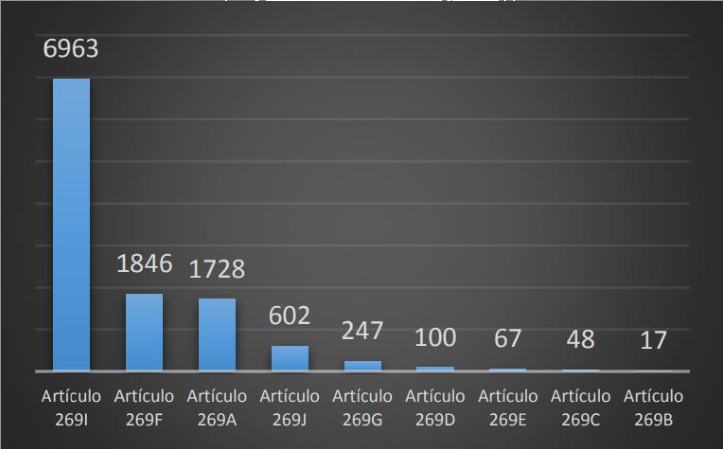
\includegraphics[width=0.75\textwidth]{./pictures/delitos.png}
  \caption{
    \textbf{Nota:} Esta gráfica representa el delito más denunciado según el
    balance del cibercrimen en Colombia en 2017, donde se habían recibido
    11.618 denuncias. Tomado de \cite{Mosquera2019}
  }
  \label{fig:delitos}
\end{figure}

\textcite{He2023}

\subsection{Diagrama de Ishikawa y conclusiones generales de los problemas}

% Por completar
\textcite{CanoMartinez2022} junto con los comentarios dados por
\textcite{Nurul2021} se identificó que la causa más común de las fallas de
seguridad de un sistema tecnológico es el engaño; independientemente de las
técnicas de ``hacking'' que se empleen, se puede llegar a lo que se desea de
una o varias personas.

Al tener en cuenta varias de las causas que provocan el inadecuado
funcionamiento de un equipo de cómputo, se sintetizan en la
Figura~\ref{fig:fish}:

\begin{figure}[htb]
  \centering
  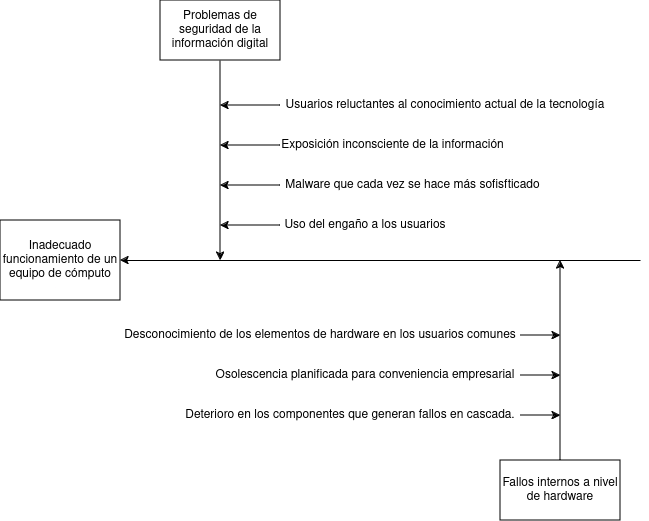
\includegraphics[width=0.9\textwidth]{./pictures/diagrama.png}
  \caption{Diagrama de Ishikawa sobre la problemática}
  \label{fig:fish}
\end{figure} 
